\documentclass{kththesis}
\usepackage[utf8]{inputenc}
\usepackage[style=ieee]{biblatex}
\usepackage{amsmath}
\usepackage{xcolor}
\usepackage{colortbl}
\usepackage{pdfpages}
\usepackage[toc,page]{appendix}
\usepackage{tabularx}
\usepackage{csquotes}
\usepackage{float}
\usepackage{pgfplots}
\usepackage[normalem]{ulem}
\useunder{\uline}{\ul}{}
\pgfplotsset{compat=newest}

\addbibresource{references.bib}

\usepackage{graphicx}
\graphicspath{ {images/} }

\usepackage{subcaption}
\usepackage{tikz}
\usepackage{pgfplots}
\usepackage{wrapfig,lipsum}
\def\rot#1{\rotatebox{90}{#1}}
\pgfplotsset{compat=1.17}
\newcommand*{\Num}{N\textsuperscript{o}\xspace}




\title{Project Specification}
\author{Jaime Ferrando Huertas }
\date{February 2018}

\begin{document}
\begin{titlepage}
 

\end{titlepage}

\begin{titlepage}
    \begin{center}
        \begin{figure}
            \centering
            \begin{subfigure}{.5\textwidth}
              \centering
              
\includegraphics[width=.7\linewidth]{logoUPV3.jpg}
            \end{subfigure}%
            \begin{subfigure}{.5\textwidth}
              \centering
              
\includegraphics[width=.7\linewidth]{2560px-H&M-Logo.svg.png}

            \end{subfigure}

        \end{figure}
        
        \vspace*{1cm}
        
        \textbf{\Large{Master thesis}}
        
        \vspace{0.5cm}
        Fashion recommender systems with focus on time and 
        seasonability.
    
        
        \vspace{1.5cm}
        Author:
        \\
        \textbf{Jaime Ferrando Huertas}
        
        \vspace{1.5cm}
        Supervisors:
        \\
        \textbf{UPV: Roberto Paredes Palacios}\\
        \textbf{H\&M: Björn Hertzberg}
        
        \vfill
        School:  \textbf{DSIC - Departamento de Sistemas Informáticos y Computación}
        \\
        University: \textbf{UPV - Universitat Politècnica de València} 
        \\
        Date: \textbf{September 2021}
        
    \end{center}
\end{titlepage}


\tableofcontents
\clearpage

\begin{abstract}
Recommender systems have a strong presence in today's web platforms, e-commerce, media platforms, news, and any platform that aims to boost user engagement through user personalized content offerings. These systems collect user information and use it to deliver personalized experiences, minimizing the overload of content while providing the most relevant content for the user. The state-of-the-art models for recommendation systems have varied during the last years. Models have transitioned from matrix factorization methods to neural-based models based on large artificial neural networks.

This thesis aims to explore such neural-based models on a big fashion retailer, H\&M. H\&M is one of the biggest fashion retailers in the world and can benefit from user personalized recommendations to improve sales and user engagement with the brand. H\&M has been using matrix factorization methods in the past. Still, these methods can not catch temporal relations such as trends or seasons, neither the time evolution in a customer fashion preferences. We will work with neural-based models that capture that can capture such information.

The data comes from the Swedish market for H\&M consists of web interactions. We will evaluate models with both traditional and diversity metrics. It is essential to assess diversity metrics in the recommendations offered. It is not always best to recommend the bestseller article, but instead recommend articles that boost user engagement, then translate into better selling.

Results indicate neural models can capture such temporal relations and perform better than the previous methods used at H\&M.
\end{abstract}
\clearpage

\section*{Acknowledgements}
For the fulfillment of this project, I would like to thank everyone at the H\&M team for their support and for allowing me to work on their recommender system. Having access to a unique recommender industrial application has been an honor. I would also like to thank my supervisors, Roberto Paredes and Bjorn, for their precious feedback, extensive discussions, and enormous help throughout the project.

I am grateful for all professors at UPV Master's Degree in Artificial Intelligence, Pattern Recognition and Digital Imaging for their great teachings during the program. I am thankful to realize an industry collaboration for my master thesis, which proves the real industry applications the program offers. Finally, none of the mentioned work would have been possible without my family's sacrifices, who believed in me during my career and supported me to work abroad, with my heartfelt gratitude.
\newline
\newline
\newline
\newline
\newline

\noindent Stockholm, August 26, 2021 \\
\noindent \textit{Jaime Ferrando Huertas}

%%%%%%%%%%%%%%%%%%%%%%%%%%%%%%%%%%%%%%%%%%%%%%%%%%%%%%%%%%%%%%%%%%%%%%
%---------------------------------------------------------------------
%%%%%%%%%%%%%%%%%%%%%%%%%%%%%%%%%%%%%%%%%%%%%%%%%%%%%%%%%%%%%%%%%%%%%%
\chapter{Introduction}

Recommendation systems are a subset of information filtering systems built to provide individualized and personalized recommendations to users in an ample space of possible options. These recommendations aim to deliver relevant offerings to the user. The systems are built with information from both the user's preferences and item space.

Thanks to the massive increase of both available data and tools to process it, these recommendation systems have gained popularity for the last few years. They saw a rise in popularity thanks to the Netflix price dataset \cite{netflix} and have been used in many business use cases such as Spotify, Youtube, Amazon, Google, or Airbnb. These use cases work in a different business market, yet they require a powerful recommender system; this is due to their large amount of offerings and the need to filter them to the user. Recommender systems will use both content and user data to filter the offerings and provide only the most relevant offerings to the user. A personalized and relevant offering of content to the user translates into more interactions.

Recommender systems can be used across different domains, but is it one type of recommender system used across all domains? or is it one type per domain? The answer to the question relies on what available data the domain has. There are different approaches to recommender systems based on the data they used. The main two types of recommendation system are \textbf{Content-based}, which examines the user's previous content interactions and the content attributes to recommend new content. \textbf{Collaborative filtering} creates a user profile based on their content interactions and recommends content that similar profiles have interacted with. Content interactions can be explicit or implicit and will determine the way we treat them.

At H\&M, we have implicit data in the form of web-based article interactions or purchases. Previous methods used at H\&M went with the collaborative filtering approach and created user profiles based on their interactions to recommend items that neighbor profiles had interacted with. With a new set of neural models, we will follow a content-based approach. We will provide user features and user-item interaction history to a model that will output a set of recommendations.

\section{Problem Statement}

In this project, we will implement a new neural-based recommender system and compare its performance to the previous matrix factorization model currently in use at H\&M.  Current implementations at H\&M do not capture time relations which are strongly present in the fashion domain, the new neural-based model will have a special architecture to facilitate learning from these relations. In particular, we will examine performance along with the following points:

\begin{itemize}
    \item Performance on next item to interact, traditional classification metrics such as Hit Ratio at K (HR@K).
    \item Diversity metrics such as Coverage, Overlap, Personalization, and novelty. These metrics allow us to evaluate recommendations from a closer perspective to the user to understand user engagement better. 
\end{itemize}

\section{Scope and objectives}

Thesis scope is to compare different set of models for our recommendation systems at H\&M with an extensive evaluation for both performance and diversity metrics. Our objective won't be to fine-tune models to achieve their best performance, but rather provide an initial performance measurement to showcase their potential.

Several metrics will evaluate each model's performance to examine both their accuracy and user engagement potential. We will provide conclusions on the results from the H\&M point of view. We will perform additional experiments to understand our model's performance, change embedding dimensions for both item and user, study length of user history, and use randomized user histories.

\section{Thesis outline}
The rest of this report is organized as follows: In the second chapter, the main background needed for understanding the report will be given. This background comprehends from recommender systems terminology to an overview of artificial neural networks and the specifics of the models we used. The third chapter explains the specific architecture of the models tested. The fourth chapter gives an overview of the training setup and data processing, with a presentation of experiments results. The fifth section discusses the presented results and the limitations of the project, finishing with future work and conclusions.

\section{Sustainability and ethics}
Recommendation systems are built to interact with users by nature, raising concerns about their ethics and responsibilities. The initial problems start with the data used to train such models. Did the users provide consent for the usage of their data to train these models? Or even just usage of the data to provide them with recommendations. Companies will often collect as much data as possible and use them on their systems. Data collection policies have raised concerns on the European Union, and regulations for users' privacy have started to appear \cite{EUdataregulations2018}. The company's responsibility is to let the user know what data is collected, how, for how long, and what it will be used to. This data will have to be stored appropriately to protect user privacy and follow necessary regulations.

The impact of the recommendation system can also raise concerns; recommendation systems can produce negative effects on users' life. After all, getting the user to interact more with the offered content is the objective. We have seen this happening with social media, where companies changed their chronologically ordered feed for user personalized feeds. This change made it possible to improve user engagement and retain them in their platform for as much as possible.

\chapter{Background}
\section{Recommender Systems}
This section will give an overview of what is needed to know about recommender systems, what types exist, and how they are built. In the introduction chapter, we mentioned how these systems can be applied to different use cases and how the data they are based on will decide the type of system to implement, now we will define the various taxonomies of recommender systems and what data they require. This will allow us to identify a fitting solution to our problem.

\subsection{Definition}
Recommendation systems are a subset of information filtering systems built to provide individualized and personalized recommendations to users in an ample space of possible options. These recommendations aim to provide a more relevant offering to the user.

To create personalized recommendations, the system needs to learn the user preferences while having all the available information on the items space. The system needs to anticipate the user's needs and present new and relevant items the user will find fitting but would not have consumed without the system proposing it.

\subsection{Recommender system types}

We now present several types of recommender systems.

\begin{itemize}
    \item \textbf{Collaborative systems} One of the most common systems, collaborative systems create user profiles based on their interactions with the content (ratings, purchases, clicks). The system will then use similarity methods to find user neighborhoods and create recommendations based on the inter-users measures. Collaborative systems can work with almost any data, explicit or implicit. These systems perform at best when the user population is high as neighborhoods will be much more populated, and the system can cover all types of users. Collaborative filtering does not take time as input and will assume people who agreed in the past will agree in the future; users will like similar content as they liked before.
    
    \item \textbf{Content-based systems}  These systems focus on the attributes of the content to create the recommendations. Content such as a cloth garment would be tagged with different attributes such as style, colour, size, sex, category. The systems will learn a user profile from the content the user has interacted with and provide recommendations based on it. Content labeling will play a significant role in the model performance, as it will determine its ability to capture inter-content relations. An example of this could be Spotify recommendations, where it will recommend songs within the same genre. 
    \item \textbf{Demographic-based systems} Demographic systems are very close to collaborative approaches in the sense that they will try to find similar users to find relevant recommendations. Still, now user similarity will not be computed on their interaction history but rather on their demographic attributes. Demographic attributes can include location, genre, profession, and other personal attributes. An example of these recommendations could be AirBnB recommending group activities for vacations based on the location and personal demographics of the group.
    \item \textbf{Knowledge-based systems} Knowledge systems are based on underlying information on the relation between user needs and content. They use the explicit knowledge of the item space together with the user preferences to create recommendations. An example of such systems could be a tourism recommender system where there are no previous interactions of the user with the visiting place, but the system matches certain activities with the user thanks to its preferences and activities knowledge.
    
    \item \textbf{Utility-based systems} Utility systems try to calculate the usefulness of the content to a specific user. This can be done by learning a user profile over time or based on user expressed preferences. An example of this recommender would be a clothing size recommender; the user will input it's desired fit and needs, and the system will find the fit with the most usefulness.
    
\end{itemize}

These are the main five types of recommender systems, each one with its advantages and disadvantages. When deciding what type of system we want to implement, we need to study the best fit. If we take the Utility-based approach, we can see how useful it can be when implemented in clothing companies. People have different clothing needs depending on the weather, but weather conditions may not play such a significant part if we were to use it in Spotify.

The available user data will play a huge role when deciding what system to use. A famous recommendation problem is the cold start \cite{coldstart} where a new user comes into the systems, user profile is blank, and you need to provide recommendations. Systems like collaborative or content-based will not have enough information to provide relevant recommendations, but demographic will as long as the user provides enough demographic attributes when signing in the system.

The mentioned taxonomies are not exclusive from one another; one could implement a mix of collaborative and content-based approaches by implemented content-based user-profiles and the collaborative approach to find inter-user content relevant to the user. One could also implement different recommender systems and then join recommendations with an ensemble approach. These join models are called hybrid systems.

\subsection{Hybrid systems}
We often see recommendation models made of joint systems that complement each other in strengths and weaknesses; these models are referred to as hybrid systems. There are multiple taxonomies to join recommender systems, but these are the most common \cite{Burke_hybrid}.

\begin{itemize}
    \item \textbf{Weighted recommender} Multiple recommender systems are implemented and joint with an assigned weight. This is the simplest hybrid system and reminds us of traditional machine learning ensemble techniques.
    
    \item \textbf{Switching recommender} Multiple systems are implemented and used at the same time; the master recommender will decide if to present all recommendations to the user or choose which system to display depending on user features. If the master presents all systems recommendations at the same time, it will be called a \textit{mixed recommender}, but if it chooses one system to display, it will be a \textit{switching recommender}.
    \item \textbf{Cascade recommender} Different systems are combined in a cascade architecture where the output of a system as input for the next system and so on. This system aims to optimize results by using multiple approaches.
\end{itemize}
\subsection{Data sources}

We have mentioned how the selection of the recommender system is highly affected by the available data sources. In this section, the most common data sources used across recommender systems are presented.

\begin{itemize}
    \item \textbf{User-Content interactions}: Data for all content interactions the user has made. These interactions could be purchasing an item, listening to a song, or rating a film. There are many types of interactions, but they are usually divided into two groups: \textit{Implicit} and \textit{Explicit}. For example, purchasing an item will let us know the user's interest in the item. Still, we do not have any measure of user satisfaction with the item - implicit interaction. If the user rates a film within a scale, we have a metric to capture the user satisfaction with the film - explicit interaction. Often explicit interactions hold more value than implicit as they represent a more real metric of user satisfaction; there are data enrichment techniques for implicit interactions to come close to an explicit interaction, let's say you listen to a song in Spotify, you are not providing any rating, but the system could capture if you listen to the full song or if you listen to it multiple times to differentiate from other interactions.
    \item \textbf{Content attributes}: Contains all data attributes related to the content the system works on. In a Spotify recommender system those could be song genre, artist, publish date, and many more.
    \item \textbf{User attributes}: All user data from demographic attributes to preferences. This data will play a significant role in systems that try to model the users as they are dependent on it. 
    \item \textbf{Functional data}: Data that could provide the system with functional requirements or information that scapes the rest of data sources. An example could be the weather forecast; a clothing recommendation system could boost waterproof items if the forecast is rainy.
\end{itemize}

\section{Recommendation techniques}
In this section, we describe the most common techniques used to create recommendation systems.

\subsection{Collaborative filtering}
Collaborative filtering approaches have been the most popular choice of recommender system in the last decade. Thanks to the massive amount of data platforms started collecting; they found techniques to model the user and find similarities in a vector space. Traditional methods use factorization to create a latent space that captures interactions between users and items.

These systems require a historical list of content interactions per user to create a user-profile that will later be used to compute distances between users. The system is highly sensitive to the number of interactions and can be extremely affected by the cold-star problem with new users. Another caveat of these systems is the high sparsity in the user-item matrices.

\subsubsection{Nearest neighbours}
A technique used both on user-based and item-based neighborhood methods. The system creates a similarity between users and finds the nearest neighbors to the current user to find content neighbors interacted with. The utility of an item $s$ for a user $c$ in can be estimated as \cite{knn}:

\begin{equation}
\hat{u}_{c, s}=\frac{\bar{u}_{c}+\sum_{c^{\prime} \in N_{c}}\left(u_{c^{\prime}, s}-\bar{u}_{c}^{\prime}\right) \times \operatorname{sim}\left(c, c^{\prime}\right)}{\sum_{c^{\prime} \in N_{c}} \operatorname{sim}\left(c, c^{\prime}\right)}
\end{equation}

Where we have K nearest neighbors of user $c$ in $N_c$, $\bar{u_c}$ the mean utility of previous items the user has interacted with and $sim(c_1,c_2)$ being a similarity measure between users such as cosine similarity, Pearson correlation or any dimensional similarity measure.


\subsubsection{Matrix Factorization techniques} \label{als}
Techniques that become popular after the Netflix Price \cite{netflix}. A competition on collaborative filtering methods was won with such techniques. Matrix factorization techniques present a new approach to solve the high sparsity in traditional collaborative methods. Netflix's competition was won with Matrix Factorization methods \cite{matrix}. These methods split the user-item matrices into multiple smaller matrices. The user-item interaction matrix is split into two lower dimensional matrices, the first one has a row for each user, and the second has a column for each item. Each row or column corresponding to a user or item will be referred to as latent factors \cite{latentspace} that will create a latent space.


\begin{figure}[H]
    \centering
    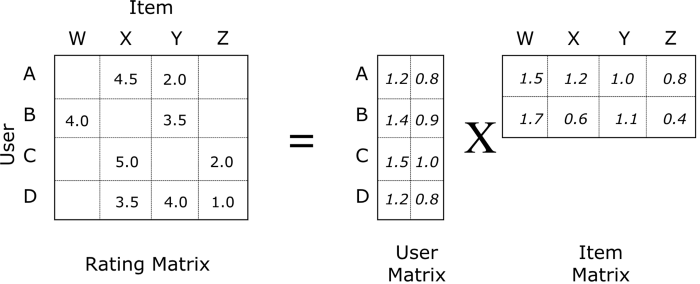
\includegraphics[width=\textwidth]{matrix_factorization.png}
    \caption{Matrix factorization example for a movie ratings dataset.}
\end{figure}

In the first implementation applied to the Netflix Price \cite{matrixvanilla} we find the predicted rating per each user $u$ for a given item $i$ is defined as follows:

\begin{equation}
    \tilde{r}_{u i}=\sum_{f=0}^{n \text { factors }} H_{u, f} W_{f, i}
\end{equation}

Ratings can be computed as:
\begin{equation}
    \tilde{R}=H W
\end{equation}

Where $\tilde{R}$ is the user-item matrix, $H$ contains user latent factors, and $W$ the item latent factors. Such logic is referred to as the original matrix factorization method, but several other optimizations have been raised since then with SVD \cite{svd}, and ALS \cite{alsnetflix}. Alternating Least Square (ALS) has been a dominant approach thanks to its parallel computation approach.


\subsubsection{Neural based}
With the rise of neural networks in different fields, they also reached recommendation systems \cite{neuralonrecommendations}. Deep learning methods have been developed to tackle the collaborative filtering approach. There has been proposed methods based on denoising autoencoder networks \cite{wang2015collaborative}. Still, it was not until Deep Item-based Collaborative filtering \cite{deepicf} that deep learning methods beat traditional techniques. DeepICF made use of attention layers which already revolutionized the natural language field \cite{attention}. 

Deep learning methods performed well in recommendations because of their power to find good items and user representations in the embedding space. Embedding layers have been used previously in natural language processing and revolutionized the field due to the dramatic decrease in sparsity to represent words and their accurate representation. 

\subsection{Content based}
Content-based recommender systems are built around item attributes and user profile preferences. The basic idea is to recommend items that are similar to what the user liked before \cite{contentbased}. These methods are suitable for situations with extensive data about the items and do not require user attributes such as demographic data. The model will build a user preference profile based on the history of its interactions and use it to recommend items the user will like.

\subsubsection{Vector Space Model}
The Vector Space Model \cite{vectorspacemodel} is the most famous method for content-based recommenders. The model inspires information retrieving systems to implement an item scorer. It treats item attributes as keywords and uses the TF-IDF \cite{tfidf} to calculate weights based on those keywords. Given an item, $d_j$, its content is defined by a set of weights $w_ij$ where each weight corresponds to the $i$th keyword of the item $d_j$.
\begin{equation}
\operatorname{Content}\left(d_{j}\right)=\left\{w_{1 j}, w_{2 j}, \ldots\right\}
\end{equation}

Content-based systems will recommend items similar to what the user previously liked. To do so, it will create a user profile based on the history of items \cite{contentprofile}.

\begin{equation}
\text { ContentBasedProfile }(u)=\frac{1}{|N(u)|} \operatorname{sum}_{d \in N(u)} \text { Content }(d)
\end{equation}

Where $N(u)$ is what the user $u$ previously liked. Once we calculate the \textit{ContentBasedProfile} for all users, we can create a score $p(u,d)$ to predict what a user $u$ will give to the item $d$.

\begin{equation}
p(u, d)=\operatorname{sim}(\text { ContentBased Profile }(u), \operatorname{Content}(d))
\end{equation}

Where $sim$ is a similarity measure like Pearson correlation or cosine distance.
These systems will be highly dependent on the keywords (item attributes) available for the items. The more accurate attributes to describe the item space, the better the models will perform.

\subsubsection{Neural based}
Neural-based models bring a new approach to item representations \cite{content-embeddings} thanks to their embedding layers. Item representations can be learned without specific attributes. In \cite{spotifyembeddings} Spotify learns songs embeddings from the sequence they are present without the need for song attributes such as genre or artist.

Neural-based approaches will treat the problem as a regular classification situation and use artificial networks to predict the next item the user will like based on both user and item embeddings. In \cite{rnn-youtube} we see a basic RNN approach to the YouTube recommendation system; the system receives the user video history as an ordered sequence and predicts the next video to watch. Later on \cite{rnn-youtube-improved} they improve the model with additional context features. Other approaches for click rate prediction with attention encoders have been implemented by Alibaba \cite{alibaba}.





\section{Artificial Neural Networks}
Artificial Neural Networks (ANN) are computing models inspired by the biological neural network in animal brains. An ANN is based on a group or compute units called neurons, similar to neurons in the biological brain. These systems are often applied in pattern recognition \cite{pattern-bishop} problems such as data analysis, information retrieval, classification, regression, or computer vision. ANNs mimic the animal brain and learn from examples and do not need specific task programming, which is why they have seen a rise in popularity and the massive amount of data in the digital world. Here is an example of an ANN diagram

\begin{figure}[H]
    \centering
    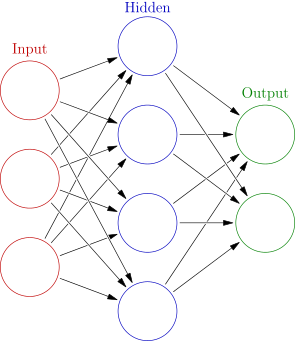
\includegraphics[scale=0.50]{Colored_neural_network.png}
    \caption{Example of a simple ANN.}
\end{figure}

The neurons building an ANN are compute units that receive one or more inputs, weightily sums them, and apply an activation function dependent on the sum to produce an output that other units can use. These units are connected in levels (layers) to form an ANN, also called fully connected networks. 

\begin{figure}[H]
    \centering
    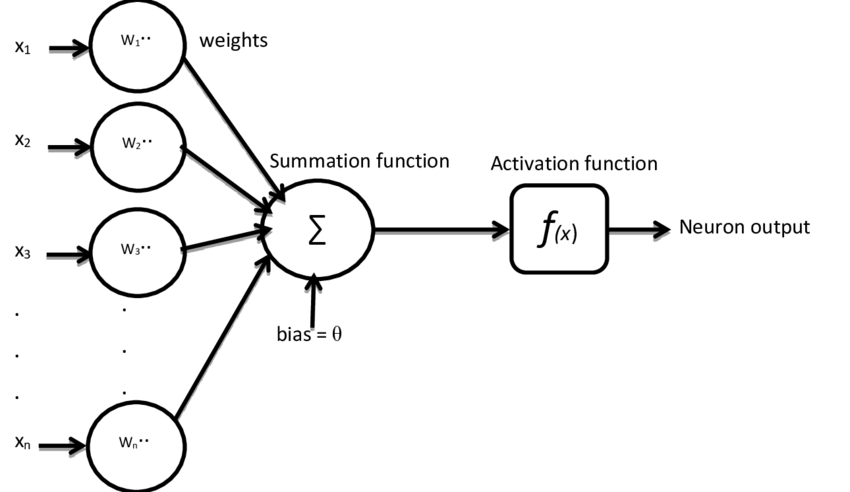
\includegraphics[width=\textwidth]{The-structure-of-the-artificial-neuron.png}
    \caption{Artificial neuron diagram \cite{neuron-diagram}. }
\end{figure}


When creating an ANN, the activation functions of the neurons will play an important role, many mathematical functions have been used in the field, but not all will fit the requirements for each use-case. The most common activation functions are RELU, Leaky-RELU, Identity or Sigmoid \cite{neurons} but there are others such as Gaussian, Hyperbolic tangent, Binary, or GELU. Here are the most common functions

\begin{figure*}[h]
    \centering
    \begin{subfigure}[b]{0.475\textwidth}
\centering
$$
f(x) = \begin{cases}0 & \text { if } x \leq 0 \\ x & \text { if } x>0\end{cases}
$$
\caption{Rectified linear unit (ReLU)\cite{relu}}
    \end{subfigure}
    \hfill
    \begin{subfigure}[b]{0.475\textwidth}  
\centering
$$
\begin{cases}0.01 x & \text { if } x<0 \\ x & \text { if } x \geq 0\end{cases}
$$
\caption{Leaky RELU \cite{lrelu}}
    \end{subfigure}
    \vskip\baselineskip
    \begin{subfigure}[b]{0.475\textwidth}   
\centering
$$ f(x) = x$$
\caption{Identity}
    \end{subfigure}
    \hfill
    \begin{subfigure}[b]{0.475\textwidth}   
\centering
$$ f(x) = \frac{e^{x}}{e^{x} + 1}$$
\caption{Sigmoid function}
    \end{subfigure}
    \caption[  ]
    {\small Most common neuron activation functions} 
\end{figure*}
    
Every set of weights in a neuron layer are learnable during training. Weight training is the foundation of neural networks training, and while there are multiple mathematical techniques to learn them, most common one is Backpropagation \cite{backprop}. In Backpropagation we need an error function to evaluate how well the current weights are performing, for example, the RMSE error for a regression problem. We will derive our learnable weights against that error function to travel within the hyperplane of weight values, finding the ones with the lower error function. This algorithm is computed inversely; the output layer errors are calculated first and then propagated to the previous layer to compute their errors. The process is repeated until reaching the first layer.

\subsection{Feedforward Neural Network}
Feedforward neural networks (FFNN) are the basic iteration of ANN where neurons can only be connected forward, not establishing a connection with themselves or previous neurons. Information will only move forward, starting from the input layer to the hidden layers and finally the output layer. A diagram of FFNN can be seen here:

\begin{figure}[H]
    \centering
    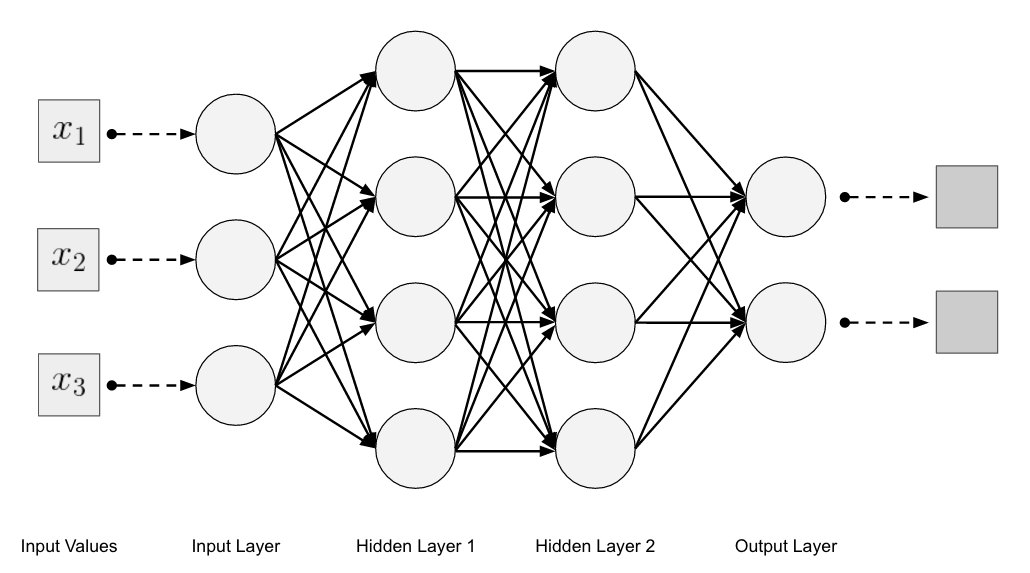
\includegraphics[width=0.6\linewidth]{fnn.png}
    \caption{Example of a FFNN \cite{ffnn}.}
    \label{FFNN}
\end{figure}

These networks are often referred to as multilayer perceptrons and created the foundation of neural networks today.

\subsection{Recurrent Neural Networks}

Recurrent Neural Networks (RNN) are a class of ANN where connections between neurons can form a directed graph. Cycles are formed in the neuron connections, where a neuron receives its own output. RNNs are commonly used to process sequences of inputs with variable length, as they create an internal state(memory) and process each input sequentially, capturing sequence relations. This makes them specially useful for task as handwriting recognition \cite{rnn-hand} and speech recognition \cite{rnn-speech}. Here we can see a diagram of an RNN cell.

\begin{figure}[H]
    \centering
    \includegraphics[width=\textwidth]{images/RNN_core.png}
    \caption{RNN cell \cite{daniel}}
    \label{RNN}
\end{figure}

The cell receives both the input vector $x_{t}$ and the previous hidden layer vector $h_{t-1}:$ and behaves as a standard neuron.

\subsection{Long short-term memory - LSTM}
Long short term memory(LSTM) ANN are a special RNN architecture \cite{lstm-author}. LSTMs replace RNN neurons by LSTM cells where that are is composed of three gates:
\begin{itemize}
    \item Input gate
    \item Output gate
    \item Forget gate
\end{itemize}

Each of the gates can be treated as a single neuron. Thanks to the more elaborate architecture, LSTM cells can learn time dependencies and makes them especially useful for time series, machine translation, or any use case where time plays a role. Generally, RNNs are outperformed by LSTMs. Here we can see a diagram of an LSTM cell.

\begin{figure}[H]
    \centering
    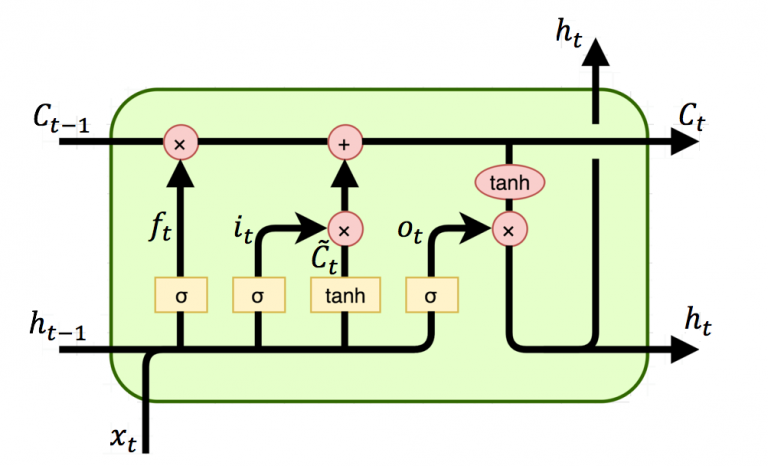
\includegraphics[scale=0.6]{LSTM-Core.png}
    \caption{LSTM cell diagram  \cite{daniel}.}
    
\end{figure}

The cell receives the input vector $x_{t}$, previous hidden layer vector $h_{t-1}:$ and the previous cell state $c_{t-1}$. From left to right, forget gate $f_t$, input gate $i_{t}$, cell state candidate values $\bar{C}^{(t)}$ and output gate $o_{t}$. All the elements will control the flow of the input data through the cell by adding or removing information from the cell state$C^{(t)}$.

\subsection{Gated recurrent unit - GRU}
A Gated recurrent unit (GRU) \cite{gru} is another type of RNN architecture similar to LSTMs. GRU cells have two gates, a reset gate \cite{gru-forget}, and an update gate. The reset gate determines how to combine the new input with the previous memory, and the update gate defines how much of the previous memory to maintain. If the rest gate is set to 1 and the update gate to 0 it will be equivalent to a plain RNN.

GRUs have seen better performance than LSTMs in speech recognition task \cite{gru-speech}, but it is still unclear which cell performs best. Here we can see a diagram of an LSTM cell. 

\begin{figure}[H]
    \centering
    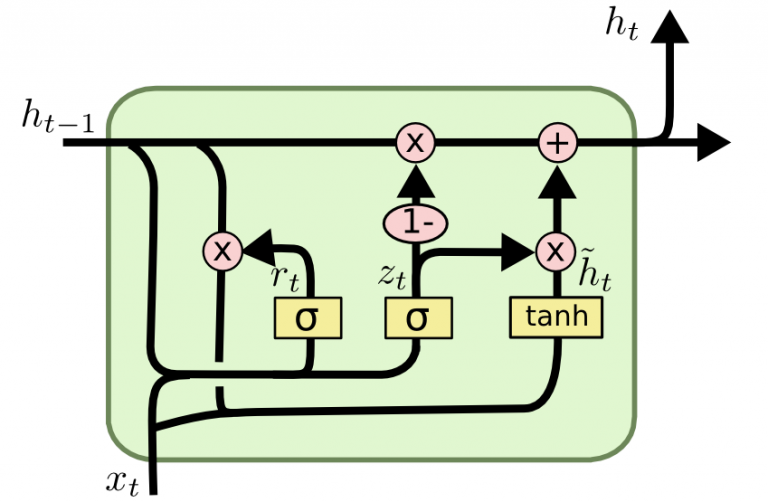
\includegraphics[scale=0.6]{GRU-core.png}
    \caption{GRU cell diagram \cite{daniel}.}
    
\end{figure}

The cell receives the input vector $x_{t}$ and previous hidden layer vector $h_{t-1}:$. Reset gate $r_t$ and update gate $z_t$ will determine the flow of input data that the cell receives.

\subsection{Encoder-decoder architectures}
The encoder-decoder (enc-dec) architecture is an ANN architecture widely used for tasks where sequences are mapped to another sequence, such as machine translation or speech recognition \cite{encoder-decoder}. The network is composed of one encoder and one decoder. The encoder transforms each item into a corresponding hidden vector containing the item and its context. The decoder reverses the process, turning the vector into an output item, using the previous output as the input context.

\begin{figure}[H]
    \centering
    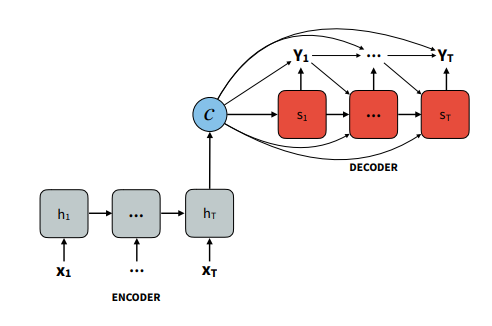
\includegraphics[scale=0.6]{encoder.PNG}
    \caption{Encoder-decoder diagram \cite{attentionplots}.}
\end{figure}

These architectures have received many optimizations such as attention layers, beam search for decoders. They were the bases for transformers models, the current state of the art for deep learning machine translation and speech recognition models.

\subsection{Attention}
The attention mechanism was introduced in machine translation by \cite{attention} and iterates on the encoder-decoder architecture. While in the original enc-dec implementation, the decoder will transform the entire input sequence into one fixed vector, which is then passed to the decoder. The attention architecture allows the model to store all hidden states of the decoder that are then passed to the decoder. The decoder will use all previous hidden state vectors in the form of a weighted sum that passes into each decoder step. The weights of each step of the decoder are decided by a trainable layer referred to as the alignment model. Other suggestions to modify the alignment model have been made, with the dot product attention of the decoder hidden states and decoder states being the most popular.

\begin{figure}[H]
    \centering
    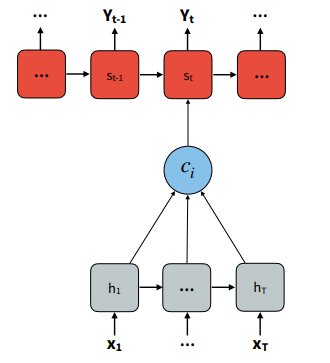
\includegraphics[scale=0.6]{enc-dec-attention.PNG}
    \caption{Encoder-decoder with attention diagram \cite{attentionplots}.}
\end{figure}


\subsection{Transformers}\label{Transformers}
Transformer models are based on the encoder-decoder architecture and add multi-head attention mechanisms in both encoder and decoder. With transformers, both encoder and decoder can consist of multiple sequentially connected blocks. Transformer models are the current state of the art in natural language processing.

\begin{figure}[H]
    \centering
    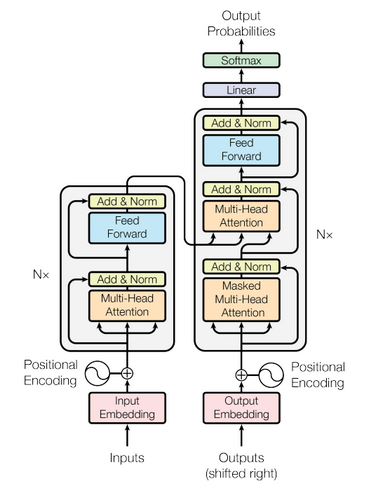
\includegraphics[scale=0.6]{transformer.PNG}
    \caption{Transformer model architecture \cite{attentionisallyouneed}.}
\end{figure}

The encoder has $N$ sequentially connected blocks. The first block receives an input vector along with its positional encoding to form the encoder input. The encoder input goes through multi head attention and a feed forward layer. Output will be sent to the next encoder block or decoder if it's the last encoder block. 

Each transformer encoder consists of two parts: multi-head attention and a feed-forward layer. The attention mechanism receives inputs from the previous encoder and processes them in a feed-forward layer to create the output encodings. Each output is individually processed by the feed forward layer and is sent to the next encoder and all decoders. The first encoder also receives positional encodings to respect each input position in the sequence; this is necessary as there is no other information about the sequence order.

The transformer decoders have three main parts: masked multi-head attention, multi-head attention, and a feed-forward layer. The masked attention will process the decoder inputs and send them to the next multi head attention that also has all encodings. Last attention outputs will be processed by a feed-forward layer similarly to the encoder. The first decoder will also receive positional encoding to respect each input in the sequence.

After the last decoder block, the original transformer implementation had a set of linear layers and a softmax layer to produce output probabilities over the vocabulary.

\section{Natural language processing}
We have provided an overview of neural-based models used in Natural Language Processing (NLP), in which we will base our experimentation to create recommender systems. These models also used techniques from traditional NLP that allow them to create word representations, especially important as reducing input sparsity improves model's performance. For our proposed models, we will also use such techniques to learn item representations. Better content representations will come in handy for content base models, as they depend highly on content attributes.

\subsection{Word Embeddings}\label{Embeddings}
Previous methods to represent words such as one-hot encoding suffered from a high dimensionality and sparsity problem. Word embeddings appear to solve those problems in the form of a real-valued vector to represent words. Embeddings should encode the meaning of the word based on their meaning, words with similar meanings should be closer in space.

Word embeddings were originated before neural networks \cite{embeddingsPre1, embeddingsPre2, embeddingsPre3}. Still, it was not until Word2vec \cite{word2vec} that they become popular as they enabled neural networks to process natural language datasets and exploded their potential. Word embeddings can be learned in two different ways, both based on context information.

\begin{figure}[H]
    \centering
    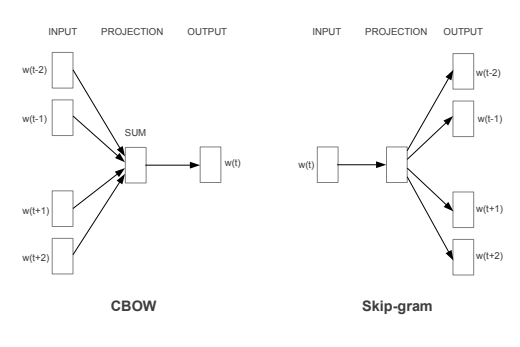
\includegraphics[scale=0.6]{word2vec.PNG}
    \caption{CBOW and Skip-gram diagrams \cite{word2vec}.}
\end{figure}

The first model, continuous bag of words (CBOW) receives a window of the surrounding context's word to predict the current word. Skip-gram in the other hands uses the current word to predict the surrounding window of context words.


\section{Evaluation}
This section provides a brief overview of what metrics are commonly used when evaluating recommender systems. We provide two sets of metrics to evaluate both the performance and diversity rate of a recommendation system.
\subsection{Performance metrics}
Performance metrics measure how good our recommender system is at predicting the content the user will consume. They provide an objective measurement of how accurate offering the recommendations are against the test data. We will be using precision at K for our evaluation, but there are other relevant metrics as NDCG, also known to be used in recommendation systems evaluation.

\subsubsection{Hit Ratio at K}
Hit Ratio at K measures the precision of the recommendation up to K recommendations. Hit Ratio is defined as the
number of correctly predicted items divided by the number of predicted
items, which is K. It's calculated as follows

\begin{equation}
\text { Hit Ratio@k }=\frac{\text { true positives } @ k}{(\text { true positives } @ k)+(\text { false positives } @ k)}
\end{equation}

This metric does not measure how accurate recommendations are ranked; it will not matter whether a recommendation is ranked 1 or 5 as long as it is within the top K. This measure is commonly referred to as precision at K (P@K)

% \subsubsection{Discounted Cumulative Gain at K}
% Discounted cumulative gain (DCG) comes from web search engines and measures the ranking quality. DCG measures the relevance of the recommendation set based on the individual recommendations relevance and their position in the result list. DCG can measure how many relevant recommendations are in the result list (how many did the user consume, similar to precision) along with their positioning on the list, helping the model improve ranking. To calculate DCG@K we use the following formula.

% \begin{equation}
% \mathrm{DCG}_{\mathrm{K}}=\sum_{i=1}^{K} \frac{r e l_{i}}{\log _{2}(i+1)}=r e l_{1}+\sum_{i=2}^{K} \frac{r e l_{i}}{\log _{2}(i+1)}
% \end{equation}

% Where $rel_{i}$ measures the relevance of recommendation $i$ in the top-K set. While in search engines, documents can have different relevance, in recommendation systems it is common to grade all user consumed content equally and set unconsumed content to zero.

\subsection{Diversity metrics}
Recommendation systems have been traditionally evaluated with performance metrics as the ones explained previously, but there is an increasing realization that accuracy alone might be a suboptimal strategy for a successful user experience \cite{noveltyintro}.
Diversity metrics complement performance metrics and provide a deeper view of how recommendations are distributed. A recommendation model could achieve good performance by simply recommending the top consumed content, but we could create a more tailored experience for the user. In the case of H\&M, recommending top-selling articles such as white shirts, white socks may show good performance metrics on paper, but it won't translate into greater user engagement. Was the user going to buy white shirts anyway, as they are the most popular item? How does the user feel when receiving non-personalized recommendations? These metrics allow us to evaluate closer to the user perspective and achieve a better user experience.

\subsubsection{Overlap at K}
Measures the percentage of unique recommendation sets in the full recommendation list. If we had a thousand users with their own recommendation set, the value would be 1 if all users got a distinct recommendation set and 0 if they all received the same recommendation set. We will use $1-Overlap@k$, and it's calculated as follows. 

\begin{equation}
\text { Overlap@K }= 1 -  \frac{\mathrm{N}^{\circ} \text { of distinct of recommendation sets }}{\mathrm{N}^{\circ} \text { of recommendation sets }}
\end{equation}

This metric is especially useful to measure how \textit{personalized} our recommender is and detect when it is overfitting to a certain set of recommendations. 
\subsubsection{Personalization at K}
Personalization at K measures uniqueness from all recommendations sets the system creates. While Overlap@K measures uniqueness in binary (unique or not unique) Personalization@k measures a more complex similarity, we calculate the dissimilarity (1- cosine similarity) across all user's recommendations. User recommendations are encoded in a vector representing whether the user recommendation included or not all possible items. We calculate the Personalization@K as follows:

\begin{equation}
\begin{aligned}
\text { Personalization@K } &= 1 - \text{mean cosine similarity} \\
&= 1 - mean(\sum_{i \in U}\sum_{j \in U}c(i,j))
\end{aligned}
\end{equation}

Being $U$ the full set of users recommendations and $c(i,j)$ the cosine similarity between vectors $i$ and $j$. This metric provides a view on how distant are the unique sets of recommendations between them.


\subsubsection{Novelty at K}
Novel recommendations are referred to as content the user did not know about \cite{noveltyintro}, novelty at K aims to measure the novelty score of a recommendation list. Recommender systems can not accurately know if the content was unknown to the user, so they assume the less popular an item is, the more novel to the user it will be \cite{noveltyassumption}. We can calculate novelty at top-K recommendations by summing the novelty of each recommendation based on its popularity. 


\begin{equation}
\text { Novelty@K }=\frac{1}{|R|} \sum_{i \in R} P O P_{i}=\frac{1}{|R|} \sum_{i \in R}-\log (p(i))
\end{equation}

With $R$ being the set of top-K recommendations and $p(i)$ a function to determine the popularity of a recommendation item. at H\&M we calculate popularity as the number of sales the item has.

\subsubsection{Coverage at K}
Coverage at K measures the percentage of items that the model covers in its recommendations. It's often measured across all user recommendations the model can create, as measuring it in a single user recommendation result would not have much sense. We can calculate it as follows:

\begin{equation}
\text { Coverage@K }= \frac{\text{\Num  of distinct content in recommendation}}{\text{Total \Num  of distinct content}}
\end{equation}


All these metrics can also be calculated on content attribute level for more detailed analysis. At H\&M we often calculate these metrics also on a category level to understand what categories our customers are receiving in their recommendations and intervene if they non-desirable results, for example, only home items 


%%%%%%%%%%%%%%%%%%%%%%%%%%%%%%%%%%%%%%%%%%%%%%%%%%%%%%%%%%%%%%%%%%%%%%
%---------------------------------------------------------------------
%%%%%%%%%%%%%%%%%%%%%%%%%%%%%%%%%%%%%%%%%%%%%%%%%%%%%%%%%%%%%%%%%%%%%%
\chapter{Models}
In this section, we will go over the different model architectures evaluated. We start with the current model at H\&M and add new neural architectures based on NLP models. NLP Neural-based architectures do a fantastic job capturing time and order relations within a sequence. We expect the same when moving them in the recommendation system usage.

\section{Baseline - AALS}
AnnoyAlternatingLeastSquares (AALS) is a matrix factorization method. Following the algorithm described at \ref{als} we will build matrices for both user and items containing the latent factors. We will use Approximate Nearest Neighbour Search \cite{annoy} (ANNOY) within the matrices to find the approximate closest neighbors in order to create recommendations. We use ANNOY and not the correct Neighbours to save computational cost, these models are trained daily, and computational time takes a role.


\section{Neural Sequencer RNN}
Basing on Google's work with Youtube recommendations \cite{rnn-youtube} we implemented a similar model adapted to H\&M use case. This Neural Sequencer RNN (N.S RNN) model consists of two embedding layers, a multi-layer RNN and a final classification linear layer. The model takes user id and user web browsing history as a sequence to predict the next item the user will interact with. Embeddings have a 256 size, RNN layers have 512 neurons and the final linear layer has 512 (twice the embedding size due to the concat layer). 

\begin{figure}[H]
    \centering
    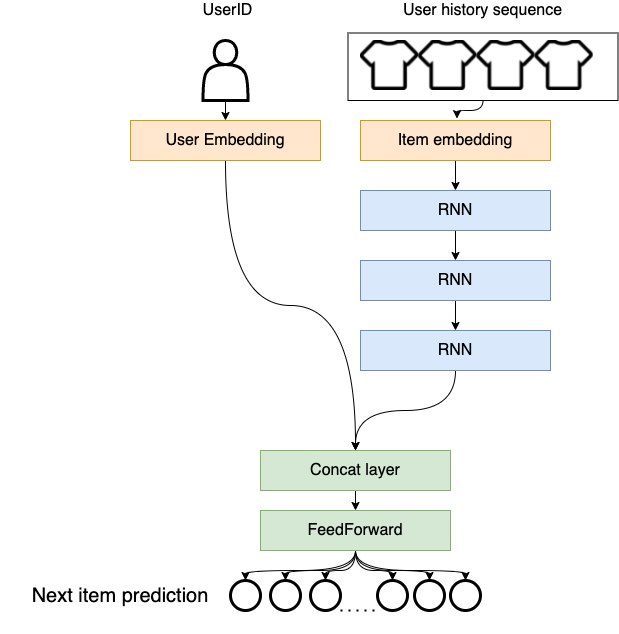
\includegraphics[scale=0.45]{images/models/RNN.png}
    \caption{Neural sequencer RNN schema.}
\end{figure}

The user id and user sequence of item interactions will pass through their respective embedding layers. The sequence of item representations will then pass through a three-layer LSTM which latest state will be concatenated to the user id representation and finally sent to a final classification layer predicting the next item the user will interact with. RNN gates are known not to be the most efficient gate for recurrent networks. We will also try another two variations with both LSTM and GRU cells.

\section{Neural sequencer with attention}
Following NLP research, our next experiment consists of the addition of an encoder-decoder architecture with attention. The attention layer was a breakthrough on machine translation \cite{attention}. Schema of the model.

\begin{figure}[H]
    \centering
    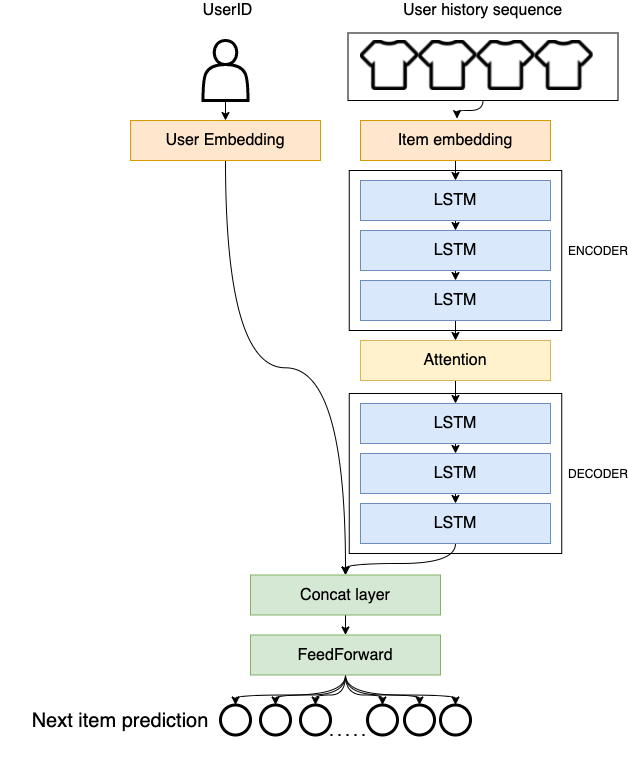
\includegraphics[scale=0.45]{images/models/Attention.png}
    \caption{Neural sequencer Transformer schema.}
\end{figure}

In the attention model, we expand upon the N.S RNN. We use the three initial layers as an encoder that passes its hidden states to an attention layer connected to a three-layer LSTM decoder which is connected to the initial concat layer. All LSTM layers have 512 neurons

\section{Neural Sequencer with transformers}
Transformers have been state of the art in NLP during the last years since \cite{attentionisallyouneed} and will be evaluated for our use case as well. We will implement a transformer recommendation architecture similar to how Alibaba created the Behavior-Sequence-Transformer model \cite{alibaba} based on user history sequences. The implementation only uses transformer multi-head attention encoders and replaces the transformer decoders with feed-forward layers without attention.

\begin{figure}[H]
    \centering
    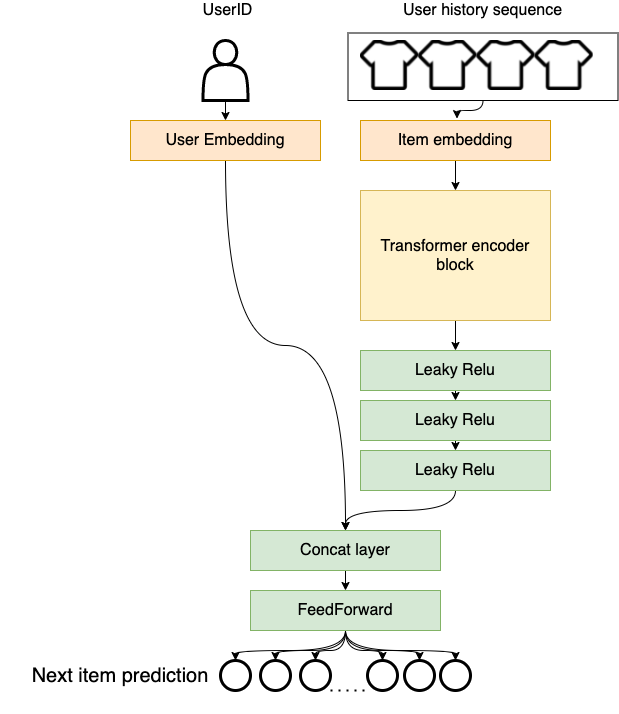
\includegraphics[scale=0.45]{images/models/Transformer.png}
    \caption{Neural sequencer RNN schema.}
\end{figure}

The transformer encoder block consists of 8 attention heads with 2048 neurons on feed-forward layers (Alibaba implementation). Next leaky Relu feed-forward layers also follow Alibaba implementation with a 1024-512-256 neuron setup.


%%%%%%%%%%%%%%%%%%%%%%%%%%%%%%%%%%%%%%%%%%%%%%%%%%%%%%%%%%%%%%%%%%%%%%
%---------------------------------------------------------------------
%%%%%%%%%%%%%%%%%%%%%%%%%%%%%%%%%%%%%%%%%%%%%%%%%%%%%%%%%%%%%%%%%%%%%%

\chapter{Experimentation and results}\label{results}
In this section, we will go over multiple experiments to understand each recommendation model performance and how both learn representations and time relations play a role in models performance.
\section{Training setup}
The main objective for the thesis has been evaluating different neural-based models. To keep a consistent training environment, we decided on some common training practices across all experiments. Batch size has been set for 2048, Adam \cite{adam} as an optimizer and OneCycle learning rate for fast convergence \cite{onecycle}. Such settings can play a significant role in model performance and are often a full research subject. To avoid going in an extensive singular model study, we went with the most common practices. We trained all experiments for an unlimited number of epochs with a patient policy of three, meaning that we will stop training when three consecutive epochs show decreasing model performance. Reported results are on the best performing epoch at test set, looking at the top fourteen recommendations.

\section{Data}
\subsection{Source}
Models have been trained with web interaction data from H\&M Swedish website for one month. We used web interactions data and not other sources such as transactions because of the higher population on web interactions. Customers browse the website much more often than they buy items. Having a populated data source will help our models generalize better, learn better representations and overall increase performance. Deep Learning models are known to be highly dependent on the number of data being trained on.

Web interactions collect the history of items the user has seen in H\&M website. Building a recommender capable of predicting the next item to browse will help users find valuable items based on their history, increasing user satisfaction and sales.

\subsection{Preprocessing}
Neural models will be trained to predict the next user interaction based on the user history. A user history of interactions can be used to create multiple samples that train the network. Given a user history $H$ containing $h_1, h_2, .. h_n$ interactions, a training sample can be created from each interaction, $h_t$ where the past interactions $h_1, .., h_t-1$ are used as past history to predict interaction $h_t$. A representation of how preprocessing would affect a user history is shown in the following figures.

\begin{figure}[H]
    \centering
    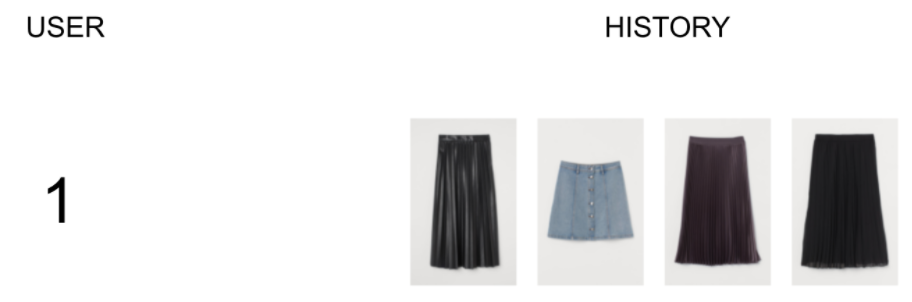
\includegraphics[scale=0.3]{images/dataset/dataset.png}
    \caption{User interaction history.}
\end{figure}

\begin{figure}[H]
    \centering
    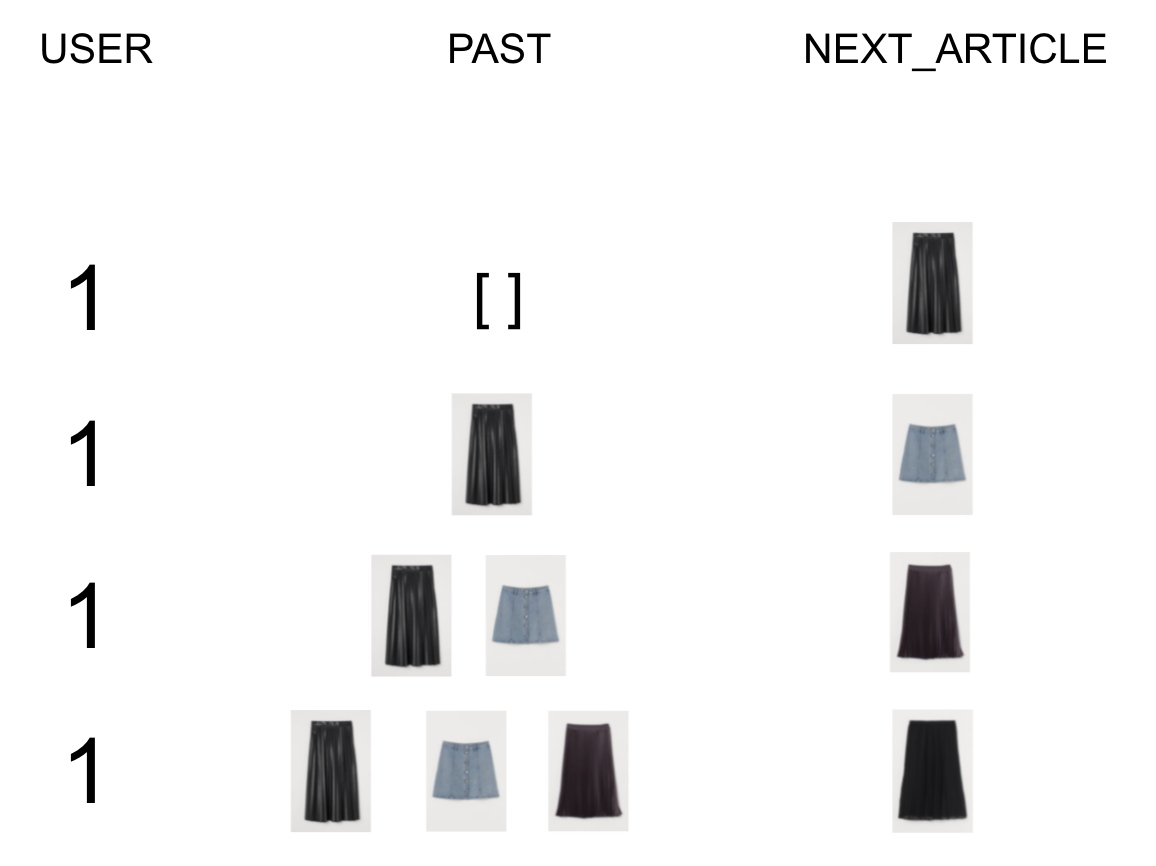
\includegraphics[scale=0.45]{images/dataset/predictionsdataset.png}
    \caption{User interaction samples.}
\end{figure}

When a user interacts with an item consecutively, $h_t-1$ will be the same as $h_t$. Consecutive duplicates interactions have been removed to prevent models from falling in local minimum scenarios where they predict the next interaction's latest known interaction.

\subsection{Split}
The training set contains all samples created from users' web history up to the second latest known interaction $h_n-1$. A test set for web history is created, where the latest interaction $h_n$ is predicted based on the previous history. We limited the test set to the latest interaction to evaluate the model at the current time and not when the model will not ever be used on. Following the preprocessing example, we can see a schema on which samples will go to training or test for the user history.

\begin{figure}[H]
    \centering
    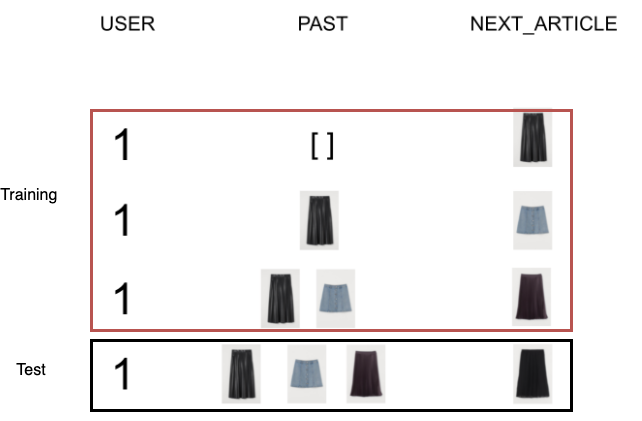
\includegraphics[scale=0.45]{images/dataset/datasetsplit.png}
    \caption{User interaction training-test split.}
\end{figure}

\section{Results}
The result of the different experiments of this project are reported below.

\subsection{Model comparisons}
Best results achieved with each of the models can be found in the following table.

\begin{center}
\begin{table}[H]
\begin{tabular}{|l|r|r|r|r|r|}
\hline
\multicolumn{1}{|c|}{\textit{Experiments}} & \multicolumn{1}{c|}{\textit{\begin{tabular}[c]{@{}c@{}}HR\\ @14\end{tabular}}} & \multicolumn{1}{c|}{\textit{\begin{tabular}[c]{@{}c@{}}Coverage\\ @14\end{tabular}}} & \multicolumn{1}{c|}{\textit{\begin{tabular}[c]{@{}c@{}}Overlap\\ @14\end{tabular}}} & \multicolumn{1}{c|}{\textit{\begin{tabular}[c]{@{}c@{}}Personalization\\ @14\end{tabular}}} & \multicolumn{1}{c|}{\textit{\begin{tabular}[c]{@{}c@{}}Novelty\\ @14\end{tabular}}} \\ \hline
AALS                                       & 4.42\%                                                                         & 0.24\%                                                                               & {\color[HTML]{333333} \textbf{14.45\%}}                                             & 56.81\%                                                                                     & 7.6                                                                                 \\ \hline
N.S LSTM                                   & \textbf{50.32\%}                                                               & \textbf{8.75\%}                                                                      & {\color[HTML]{333333} 21.54\%}                                                      & \textbf{90.57\%}                                                                            & \textbf{9.88}                                                                       \\ \hline
N.S RNN                                    & 43.94\%                                                                        & 7.68\%                                                                               & {\color[HTML]{333333} 19.84\%}                                                      & 89.87\%                                                                                     & 9.51                                                                                \\ \hline
N.S GRU                                    & 49.00\%                                                                        & 8.04\%                                                                               & {\color[HTML]{333333} 25.94\%}                                                      & 88.03\%                                                                                     & 9.45                                                                                \\ \hline
N.S Attention                              & 47.46\%                                                                        & 7.61\%                                                                               & {\color[HTML]{333333} 19.84\%}                                                      & 89.55\%                                                                                     & 9.44                                                                                \\ \hline
N.S Transformer                            & 44.33\%                                                                        & 7.67\%                                                                               & 21.97\%                                                                             & 86.98\%                                                                                     & 9.36                                                                                \\ \hline
\end{tabular}
\caption{Model results overview} \label{faketable:mul}
\end{table}
\end{center}

All the neural sequencer models obtain a much better result than the baseline model AALS in traditional metrics, around ten times the performance. An improvement was expected, but not so high. In terms of diversity metrics, neural-based models do come ahead in three out of four, they all have a much higher coverage and personalization with a small improvement in novelty. In the overlap metric, the baseline beats the neural-based models. Overlap measures the raw uniqueness of recommendation sets, while personalization captures the distance between sets. If AALS has a lower overlap and lower personalization than neural based models, this means the users have higher number of unique recommendation sets with AALS than any neural-based model but that the unique sets are not as different between them as they are in neural-based models. 

When it comes to neural-based models, the Neural Sequencer with LSTM cells pulls ahead in HR with the GRU cell version being very close. More sophisticated NLP models such as attention and transformers present lower results, but this could be due to their higher complexity and need for extensive fine-tuning. As expected, the original N.S with RNN has the worst performance. RNN was a major improvement in NLP but has been replaced for more complex cells like LSTM or GRU for some years now. Regarding diversity metrics, the N.S with LSTM cells pulls ahead again but not with a big margin, metrics within neural-based models stay fairly consistent, and we believe it is the change to neural architecture that is responsible for the improvements, not the specific tweaking to the neural architectures. 

\subsection{User representation vs Item representations}
To further extend our analysis in model performance and result explainability, we are now going to create several experiments where embedding size for both items and users is modified. We have been training with an embedding size of 256 for both. When reducing the embedding size, we reduce the model's ability to learn representations and stopping it from using them as before. The experiment will provide us insights into how dependent the model is on those representations, helping with the explainability of the results. We will use the Neural Sequencer LSTM architecture across all tests.

We first evaluate how reducing the user embedding dimensions will affect the model. We reduced up to one dimension only to push the limit on how it affects the model. 

\begin{center}

\begin{table}[H]
\begin{tabular}{|l|l|r|r|r|r|r|}
\hline
\textit{User Size} & \multicolumn{1}{c|}{\textit{Item Size}} & \multicolumn{1}{c|}{\textit{\begin{tabular}[c]{@{}c@{}}HR\\ @14\end{tabular}}} & \multicolumn{1}{c|}{\textit{\begin{tabular}[c]{@{}c@{}}Coverage\\ @14\end{tabular}}} & \multicolumn{1}{c|}{\textit{\begin{tabular}[c]{@{}c@{}}Overlap\\ @14\end{tabular}}} & \multicolumn{1}{c|}{\textit{\begin{tabular}[c]{@{}c@{}}Personalization\\ @14\end{tabular}}} & \multicolumn{1}{c|}{\textit{\begin{tabular}[c]{@{}c@{}}Novelty\\ @14\end{tabular}}} \\ \hline
1                  & 256                                     & 49.35\%                                                                        & 8.67\%                                                                               & 23.88\%                                                                             & 89.84\%                                                                                     & 9.87                                                                                \\ \hline
10                 & 256                                     & 49.92\%                                                                        & 8.72\%                                                                               & 23.62\%                                                                             & 90.32\%                                                                                     & \textbf{9.88}                                                                       \\ \hline
20                 & 256                                     & 50.28\%                                                                        & 8.74\%                                                                               & 22.53\%                                                                             & 89.92\%                                                                                     & \textbf{9.88}                                                                       \\ \hline
128                & 256                                     & \textbf{50.38\%}                                                               & \textbf{8.79\%}                                                                      & 21.58\%                                                                             & 90.44\%                                                                                     & 9.87                                                                                \\ \hline
256                & 256                                     & 50.32\%                                                                        & 8.75\%                                                                               & \textbf{21.54\%}                                                                    & \textbf{90.57\%}                                                                            & \textbf{9.88}                                                                       \\ \hline
\end{tabular}
\caption{User embedding size study on N.S LSTM}
\end{table}
\end{center}

User embedding dimension affects does not affect performance metric HR as different neural-based architectures did, but it does play a significant role in the Overlap diversity metric where we see a direct correlation when increase from 1 to 128 dimensions with 256 being similar to 128. Such behavior is understandable as overlap measures user's unique set of recommendations. With worse user representations, the model will not produce the same number of unique sets per user.

\begin{figure}[H]
\centering
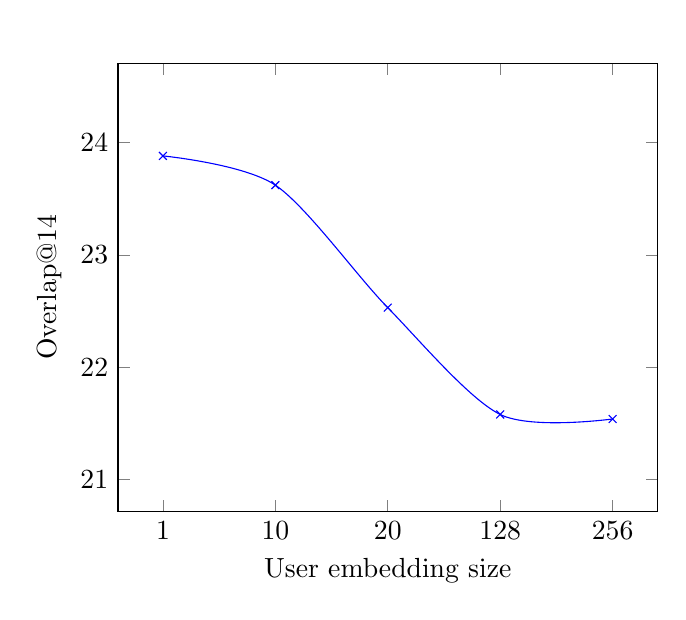
\begin{tikzpicture}
\begin{axis}[axis equal, title={\textbf{}},
xlabel={ User embedding size},
ylabel={ Overlap@14},
symbolic x coords={1,10,20,128,256}, 
xtick={1,10,20,128,256},
]
\addplot+[smooth,mark=x] plot coordinates
{ (1,23.88) (10,23.62) (20,22.53) (128,21.58) (256,21.54)};
% \addlegendentry{HR@14}
\end{axis}
\end{tikzpicture}
\caption{User embedding size length against Overlap@14}
\end{figure}

Overlap measures unique user recommendation sets so is understandable the more information the model has about distinct users the more unique the produced sets would be. For a second test, we changed the item embedding dimension:

\begin{center}
\begin{table}[H]
\resizebox{\textwidth}{!}{\begin{tabular}{|r|r||r|r|r|r|r|}
\hline
\multicolumn{1}{|l|}{\textit{User Size}} & \multicolumn{1}{c||}{\textit{Item Size}} & \multicolumn{1}{c|}{\textit{\begin{tabular}[c]{@{}c@{}}HR\\ @14\end{tabular}}} & \multicolumn{1}{c|}{\textit{\begin{tabular}[c]{@{}c@{}}Coverage\\ @14\end{tabular}}} & \multicolumn{1}{c|}{\textit{\begin{tabular}[c]{@{}c@{}}Overlap\\ @14\end{tabular}}} & \multicolumn{1}{c|}{\textit{\begin{tabular}[c]{@{}c@{}}Personalization\\ @14\end{tabular}}} & \multicolumn{1}{c|}{\textit{\begin{tabular}[c]{@{}c@{}}Novelty\\ @14\end{tabular}}} \\ \hline
256                                      & 1                                       & 35.54\%                                                                        & 6.20\%                                                                               & 22.80\%                                                                             & 89.40\%                                                                                     & 9.8                                                                                 \\ \hline
256                                      & 10                                      & 44.32\%                                                                        & 7.80\%                                                                               & 22.52\%                                                                             & 90.53\%                                                                                     & 9.82                                                                                \\ \hline
256                                      & 20                                      & 46.75\%                                                                        & 8.12\%                                                                               & 22.34\%                                                                             & \textbf{90.76\%}                                                                            & \textbf{9.91}                                                                       \\ \hline
256                                      & 128                                     & \textbf{50.87\%}                                                               & 8.34\%                                                                               & \textbf{21.32\%}                                                                    & 90.32\%                                                                                     & 9.8                                                                                 \\ \hline
256                                      & 256                                     & 50.32\%                                                                        & \textbf{8.75\%}                                                                      & 21.54\%                                                                             & 90.57\%                                                                                     & 9.88                                                                                \\ \hline
\end{tabular}}
\caption{Item embedding size study on N.S LSTM}
\end{table}
\end{center}

We now find a big impact on the HR metric; there is a direct correlation between item embedding dimension HR. Performance drops to two-thirds when items have one dimension only. Diversity metrics do see a change as well, but now in Coverage, the metric measuring the percentage of items covered in the recommendations. This drop in Coverage performance makes total sense as we are making it harder to learn item representations to the model, making it harder to distinguish them. 


\subsection{How important is an ordered sequence to the model}
One of the main hypotheses for this thesis has been to transition our recommendation model at H\&M to one that can capture time relations. After seeing an improvement in results, it is clear that the new neural-based models translate in better performance, but is it because of their ability to capture time and order relations? In this experiment, we will randomize the order of the training sequences and keep a consistent test set with the other experiments. If model performance would stay similar to the original experiments, this means it is not the time and order relations but the raw neural-based models performance that is responsible for the increase in performance. 

To study it, we tried three different orders within the user history on the N.S LSTM. 

\begin{itemize}
    \item \textbf{Correct order}: The original order in which interactions were made.
    \item \textbf{Day level order}: Randomize interactions within the same day, meaning that an interaction will only be guaranteed to be after another interaction if it happened after the second interaction day.
    \item \textbf{Random}: User history order is completely randomized.
\end{itemize}

\begin{center}

\begin{table}[H]
\begin{tabular}{|r|r|r|r|r|r|}
\hline
\multicolumn{1}{|c|}{\textit{\begin{tabular}[c]{@{}c@{}}User history\\ Sequence order\end{tabular}}} & \multicolumn{1}{c|}{\textit{\begin{tabular}[c]{@{}c@{}}HR\\ @14\end{tabular}}} & \multicolumn{1}{c|}{\textit{\begin{tabular}[c]{@{}c@{}}Coverage\\ @14\end{tabular}}} & \multicolumn{1}{c|}{\textit{\begin{tabular}[c]{@{}c@{}}Overlap\\ @14\end{tabular}}} & \multicolumn{1}{c|}{\textit{\begin{tabular}[c]{@{}c@{}}Personalization\\ @14\end{tabular}}} & \multicolumn{1}{c|}{\textit{\begin{tabular}[c]{@{}c@{}}Novelty\\ @14\end{tabular}}} \\ \hline
Correct order                                                                                        & \textbf{50.32\%}                                                               & \textbf{8.75\%}                                                                      & \textbf{21.54\%}                                                                    & \textbf{90.57\%}                                                                            & \textbf{9.88}                                                                       \\ \hline
Day level order                                                                                    & 49.37\%                                                                        & 8.04\%                                                                               & 23.39\%                                                                             & 90.46\%                                                                                     & 9.55                                                                                \\ \hline
Random                                                                                               & 43.37\%                                                                        & 7.73\%                                                                               & 22.89\%                                                                             & 85.41\%                                                                                     & 8.89                                                                                \\ \hline
\end{tabular}
\caption{User history sequence order study on N.S LSTM}
\end{table}
\end{center}

User history sequence order does play an important role in our recommendation model, affecting HR performance when having a total randomized order and with almost similar performance with a half randomize logic as the day level ordering. We also see a correlation between order and diversity metrics, with the correct order obtaining the best diversity metrics and dropping as we increase randomness in the history order.


\subsection{User history length}
How far back should we look in a user history is a big question when offering recommendations. Pasts experiments have been done with a max length of user history of twenty interactions. In this experiment, we evaluate different history lengths and how they affect our model's performance. We tried different values on the N.S LSTM and obtained the following results.

\begin{center}

\begin{table}[H]
\begin{tabular}{|r|r|r|r|r|r|}
\hline
\multicolumn{1}{|c|}{\textit{\begin{tabular}[c]{@{}c@{}}User history\\ Sequence order\end{tabular}}} & \multicolumn{1}{c|}{\textit{\begin{tabular}[c]{@{}c@{}}HR\\ @14\end{tabular}}} & \multicolumn{1}{c|}{\textit{\begin{tabular}[c]{@{}c@{}}Coverage\\ @14\end{tabular}}} & \multicolumn{1}{c|}{\textit{\begin{tabular}[c]{@{}c@{}}Overlap\\ @14\end{tabular}}} & \multicolumn{1}{c|}{\textit{\begin{tabular}[c]{@{}c@{}}Personalization\\ @14\end{tabular}}} & \multicolumn{1}{c|}{\textit{\begin{tabular}[c]{@{}c@{}}Novelty\\ @14\end{tabular}}} \\ \hline
5                                          & 45.00\%                                                                        & \textbf{8.77\%}                                                                               & 25.19\%                                                                             & 92.05\%                                                                                     & 9.41                                                                                \\ \hline
10                                         & 48.00\%                                                                        & 8.61\%                                                                               & 26.60\%                                                                             & 89.50\%                                                                                     & 9.25                                                                                \\ \hline
Default value - 20                         & 50.32\%                                                                        & 8.75\%                                                                      & 21.54\%                                                                             & 90.57\%                                                                                     & \textbf{9.88}                                                                       \\ \hline
50                                         & \textbf{50.35\%}                                                               & 7.78\%                                                                               & \textbf{16.76\%}                                                                    & \textbf{94.60\%}                                                                            & 9.69                                                                                \\ \hline
\end{tabular}
\caption{User history sequence length study on N.S LSTM}
\end{table}
\end{center}


We see a direct correlation between the max user history length and HR, the more we look back in the user history, the better our performance. We also see a major diversity impact the longer the history is, especially on the overlap metric; reaching AALS performance levels. The model can capture a more personalized representation of the history and offer a unique set of recommendations.

\subsection{Recommended items features study}
With performance or diversity metrics, we get a generalist performance evaluation, which is good enough for most of the use cases. Studying our model recommended items features provides us with a use case specific analysis on what we recommend. For H\&M we have different item attributes we look at, the first analysis is how popular are the items our models recommend. We picked our baseline model and the best performing Neural Sequencer and evaluated their popularity on the top fourteen recommended items.


\begin{figure}[H]
    \centering
    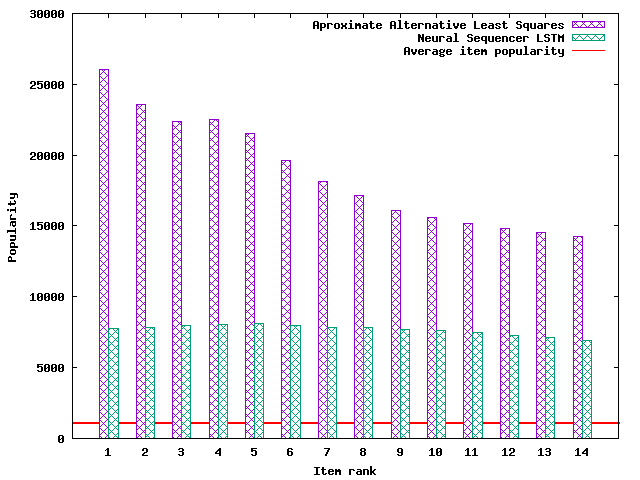
\includegraphics[scale=0.75]{charts/popularity.png}
    \caption{Average item popularity in top 14 recommendations.}
\end{figure}

Both models recommend significantly higher popular items than the average item popularity. Our baseline model is highly skewed towards high popularity items and decreases popularity as the item recommendation rank increases. The neural Sequencer model popularity stays consistant over the fourteen recommendations and stays lower than the baseline across all ranks.

Secondly, we analyze the average price on recommended items, same models and top fourteen recommended items.

\begin{figure}[H]
    \centering
    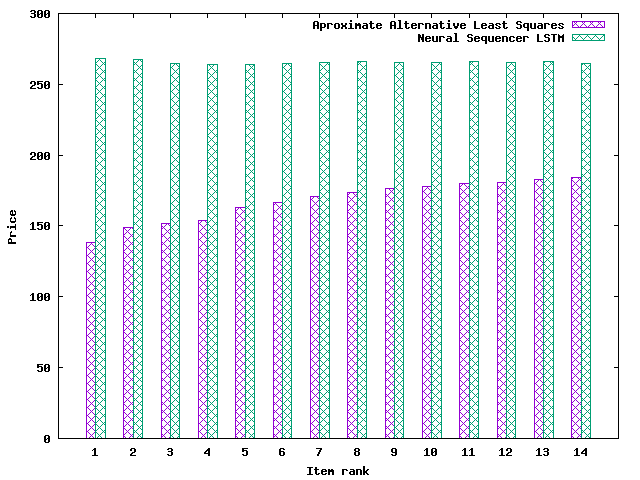
\includegraphics[scale=0.75]{charts/price.png}
    \caption{Average item price in top 14 recommendations.}
\end{figure}

Our models perform have an opposite behavior when comparing with the average item price. The baseline model recommends lower price items, while the Neural Sequencer recommends higher price items. Neural sequencer produces recommendations of almost twice the price while having better hit ratio, potentially providing higher revenue. We can connect the findings with the past analysis on item popularity, here at H&M the best-selling products are basic clothing items such as white t shirts or white packs of socks, items that are aggressively priced at very low margins. For our last analysis, we decided to evaluate the item age of the top fourteen recommended items.

\begin{figure}[H]
    \centering
    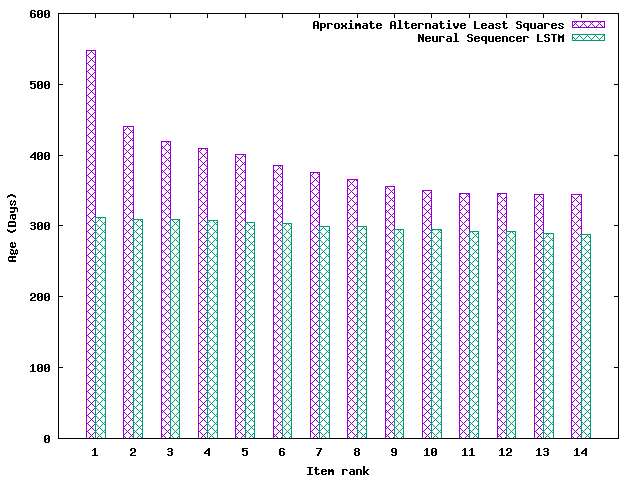
\includegraphics[scale=0.75]{charts/ages.png}
    \caption{Average item ages in top 14 recommendations.}
\end{figure}

Both models present a skew towards older items as the higher the rank they get, but in totally different scales. The baseline model presents its top tanked item with twice the age as the average item age, while the top ranked Neural Sequencer item only has $10\%$ an increase in age. The more popular items with aggressive prices are usually sold across all seasons, making them older than the on season products. 

All three analysis have confirmed our initial findings with the diversity metrics evaluation, the baseline model has a reduced set of recommended items and provides a less personalized set of recommendations than the Neural Sequencer, proved by its skew towards low-priced and popular items. We now have a business explanation on how those differences in diversity metrics are translated in offered recommendations.

%%%%%%%%%%%%%%%%%%%%%%%%%%%%%%%%%%%%%%%%%%%%%%%%%%%%%%%%%%%%%%%%%%%%%%
%---------------------------------------------------------------------
%%%%%%%%%%%%%%%%%%%%%%%%%%%%%%%%%%%%%%%%%%%%%%%%%%%%%%%%%%%%%%%%%%%%%%
\chapter{Conclusion}
\section{Discussion}
The initial objective for this thesis was to explore new models that could capture and exploit the time relations of H\&M use case to provide better recommendations than the current collaborative filtering methods. Results have shown that neural-based methods can increase both performance metrics and diversity metrics compared to our AALS methods.

We have proved the neural-based models benefit from ordering user-item interactions with our ordering experiment, with improvements not only in performance metrics but also diversity metrics as the model will have a more recent representation of the user. Experiments with the max user history length feeded to the model supported those findings and proved the importance of a good user profile representation through its history. 

We also found explainability results for our model when stress testing neural-based models with their embeddings sizes. We learned how user and item embeddings play different roles in the performance of the recommendations and can be subject to multiple optimizations. User embeddings play a bigger role in diversity metrics and do not help with performance metrics. Item embeddings are the main driver for performance metrics and the diversity metric more tied to items, Coverage.

Moreover, we failed to follow the path of NLP and Deep Learning improvements. We obtained our best performing models with recurrent networks with LSTM and GRU cells. We were unsuccessful in following the improvement's path with the usage of transformers methods as Alibaba did \cite{alibaba}.  
\cite{sun2019bert4rec}.

The thesis has served to initialize exploration of neural-based models at H\&M, providing an initial overview of how NLP methodologies can be translated to recommendations while evaluating important factors to user engagement as diversity metrics that are extremely important from the business perspective. 

There are multiple open paths to continue this work and will be treated in the future work section.

\section{Limitations}
The first limitation we found was to follow improvements in NLP models for our neural-based recommendation models. Transformers are known for requiring more fine-tuning than the methods which proved more success in our experiments. We are not sure if our results could not follow NLP path due to our implementation or due to the change of use case. While both cases have a vocabulary (words or items) NLP has much harder interrelation between the words than clothes do at H\&M. It is the addition of the user profile that makes our case drift to a new scenario where item relations take meaning inside a user context.

We mentioned how we choose approximate neighbor methods for ALS to reduce computational time. Neural-based models achieved training within one day with enough GPUs but presented a new paradigm for industrializing the models. Moving to GPU-based environments needs work, and finding people with experience on them is not as easy as with the CPU environment needed for AALS. We were surprised that GPU cloud computing costs for our models were lower than the CPU ones. We needed fewer (yet more powerful) GPU machines than CPU machines.

TOWRITEMORE


\section{Future work}
We opened multiple work paths with this thesis, and we now list what we see as the most relevant ways to continue the work at H\&M both from the academic and industrial perspectives.

\begin{itemize}
    \item \textbf{Recommendations longevity}: how our model's performance degrades over time and how it plays a role in such a fast phase industry. H\&M is a fast-fashion company, meaning that the items in stock are often replaced between seasons and do not conserve their value as they would do in other companies that aim for timeless trends or quality over looks. It is commonly known that reputable mountaineering brand's items would last and stay relevant for years, but that is the opposite of what customers at H\&M look for. There is a lot of research on recommendation use cases where items have long longevity, for example, the movie recommendations at Netflix. There is a clear research line on how the longevity of recommended items plays a role in recommendation systems.
    
    \item \textbf{Transfer learning}: Transfer learning has played an important role for NLP in recent years \cite{ruder2019transfer}. The increase in available training data and the search for reducing computational time have driven transfer learning research to a point where a lot of times, big models as BERT or ROBERTA only required little fine-tuning to specific use cases to achieve good performance. This is something to explore at H\&M as we have most of the world markets data available. The thesis project was only focused on a small market as Sweden. Can we use cross-market data to train generalist models and fine-tune them to specific markets? Can we reuse trained models within a season with little fine-tuning instead of starting from scratch every time we update the models? There could be a lot of work on finding the correct setup to use cross-market data and improve model reusability to increase both the model's performance and reduce computational cost.
    
    \item \textbf{ Split representation learning and the recommendation model}: Right now, the explored neural-based models optimize two problems simultaneously. They learn user and item representations while optimizing neural layer weights. Splitting these two optimizations problems could translate into better performance for both scenarios and provide a warm start for a final joint model. Such behavior has been seen with pre-trained word embeddings for machine translation models \cite{glove}. We have previous work at H\&M \cite{hm2vec} where we learn items representations from their images and context to find items to compose an outfit. Can such representations be used as a warm start for the recommendation models?
    
    \item \textbf{Join collaborative methods with deep learning learned representations}: Neural-based models have shown to improve our performance, but it is not clear whether the benefits come from the improved representations or the raw power of neural networks to learn distributions from data patterns. It would be interesting to explore if we can translate the learned representations to the latent space used for collaborative filtering and use known neighbor methods.
    
    \item \textbf{Deep interactions between features}: Current models use the ID from user and items to learn their representation. Work at Microsoft \cite{xDeepFM} and Alibaba \cite{alibaba} have shown how interactions from user and items to features can result in improved performance. Replacing ID embeddings for item/user feature embeddings such as age, region, category, color could benefit us with better performance and solve cold start problems where we could provide a representation to new items/users with only their attributes. Learning cross-feature relations such as user location and clothing colors can report benefits for the model.
\end{itemize}

The thesis has only been the beginning for H\&M on exploring deep learning methods applied to recommendation models. We want to continue working along with the mentioned points and provide a new perspective on how these methods can be applied for the fashion industry. 

\section{Conclusion}

The usage of Deep learning for recommendations methods is a topic with more focus coming thanks to companies like Alibaba, Amazon, Google, and other major content platforms. We have found a new niche to apply their research at H\&M. Our work proves the benefits of Deep learning at a fashion retailer, both at performance metrics and user engagement and diverse recommendations. We have identified multiple future work lines for both research and industry applications for fast phased recommendation scenarios like H\&M. Companies with access to large datasets as H\&M should explore machine learning methods as they are proving themselves as a powerful industry tool.

\printbibliography

\end{document}
